\begin{figure}[h]
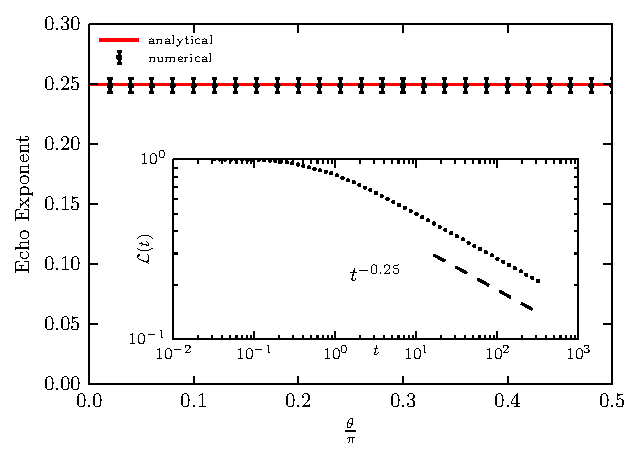
\includegraphics[width=1\columnwidth]{DDDD_fit.pdf}
\caption{The Loschmidt echo decay exponent of the process $\text{DD}+\text{DD}\rightarrow\lambda+\text{DD}$, with gluing condition $S_1(\theta)$. We work with total system size $N = 30k$ sites, and parameters $m = 10^{-8}$, $k = 1$. The lattice constant is set to unity. The blue dots representing the numerical results lie on the red analytic line. As predicted, the echo exponents are equal for different values of $\theta$. Inset: An example of Loschmidt echo with $\theta = 0.02 \pi$ shown in log-log scale. The dashline denotes the expected power law of $t^{-0.25}$. The finite size effect do not emerge before $t=10^{3}$, which sets the right boundary of the range we fit. See main text for the curve fitting method.}
\label{fig:DDDD}
\end{figure}

We use the lattice model introduced in Sec.~\ref{sec_sub:free_boson_lattice} to check the analytic results. Our numerical evaluations is based on Boson Bogoliubov transformation and explicit form of the groundstates. The readers are referred to App.~\ref{app:comp_fid_echo} for the technical details. In all the figures, we present the coefficients of the logarithmic term $\mathcal{F} / \ln L$ and $\mathcal{F} / \ln t$ and call them fidelity and echo exponents respectively. 

We start with the process
\begin{equation}
\text{DD}+\text{DD}\rightarrow\lambda+\text{DD}
\end{equation}
and shows its Loschmidt echo in Fig.~\ref{fig:DDDD}. The inset is a typical Loschmidt echo diagram, whose linear decreasing behavior in the log-log axes indicates the expected power law decay. We also provide the analytic prediction $\mathcal{L}(t)\sim t^{-0.25}$ (\cf Eq.~\eqref{eq:result_DDDD}) as a dashline for comparison. The exponent (negative of the slope of the line in log-log plot) is calculated by fitting such diagrams for $\theta = 0.02n \pi$, $n = 1,...,25 $. To avoid subjective choice of data points, we repeat 5 times to randomly pick {\color{red} 10 points} before the finite size revival surges to obtain the deviation. We see that the exponents all match with the $\frac{1}{4}$ theoretical line within error. 

We also calculate the companion process
\begin{equation}
 \text{NN}+\text{NN}\rightarrow\lambda+\text{NN}
\end{equation}
and obtain identical exponents as shown in Fig.~\ref{fig:DDDD}. The avoid the technical subtlety of zero mode by adding a small mass regulator $m=10^{-8}$. While the short time decay pattern are different from the DD case, the long time behavior and exponents remain the same for both echo and fidelity. We therefore do not present the result here. 

Next we analyze the more interesting $\theta$ dependent process
\begin{equation}
  \text{DN}+\text{DN}\rightarrow\lambda+\text{DN}
\end{equation}
in which the joining boundary condition is determined by $S_1(\theta)$. A direct calculation with the mass regulator do not perform very well in the small $\theta$ regime: the exponent is slightly larger than the theoretical prediction. We therefore turn to another regulator that shift the far end boundary condition DN to $\mathcal{S}_1( \delta \theta )$ and consider the following process
\begin{eqnarray}\begin{aligned}
\label{eq:approx_DNDN}
S_1(0)+S_1(\delta\theta)\rightarrow S_1(\theta)+S_1(\delta\theta)
\end{aligned}\end{eqnarray}
Since ${\rm DN} = S_1 (0 )$, taking smaller and smaller $\delta \theta$ should correspond to the original process. This "shift" regulator works very well for the fidelity calculation, where $\delta \theta = 0.001 \pi$, while moderately good for the Loschmidt echo, where $\delta \theta = 0.003\pi$, see Fig.~\ref{fig:DDNN}. The inset shows the $\theta$-dependence of power law decay, and the corresponding exponents follows the quadratic relation as predicted in Eq.~\eqref{eq:result_DNDN}. We leave further discussion of introducing $\delta\theta$ in Sec.~\ref{sec:disc}. 

\begin{figure}
  \centering
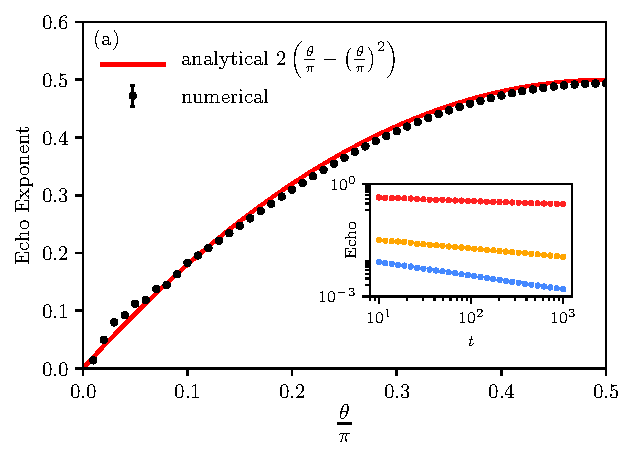
\includegraphics[width=1\columnwidth]{DDNN_fit.pdf}
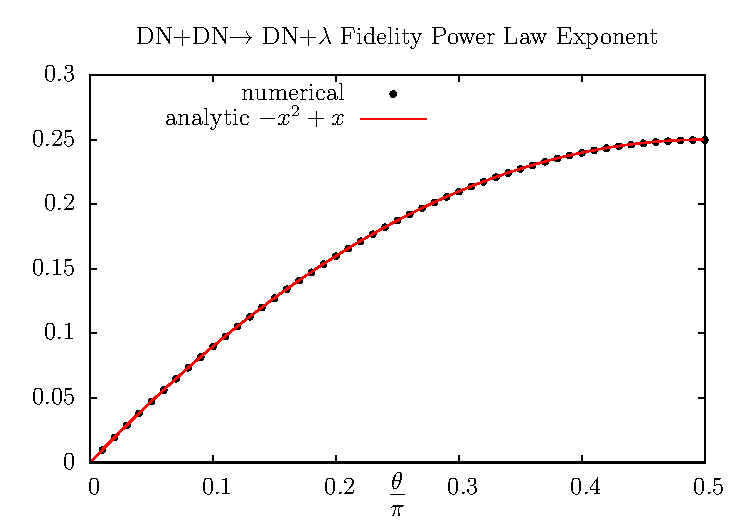
\includegraphics[width=1\columnwidth]{DN_DN2tan.pdf}
    \caption{The slope of the free energy for Loschmidt echo (a) and bipartite fidelity (b) in the process $\text{DN}+\text{DN}\rightarrow\lambda+\text{DN}$. The total system size is $N=35k$ sites with the same parameters in Fig.~\ref{fig:DDDD}. The numerical value of exponents follow a quadratic relation as predicted. There is still visible deviation from the analytic results in (a) due to the subtle zero mode, see the discussion in the main text. Inset in (a): From the top to bottom, we show the power law decay of Loschmidt echo with $\theta=0.02\pi, 0.12\pi, 0.24\pi$ and $0.48\pi$. The finite size effect do not emerge before $t=10^{4}$. We use the same curve fitting method as described for Fig.~\ref{fig:DDDD}.}
      \label{fig:DDNN}
    \todo[inline]{Tianci: make the plots have the same style?}
\end{figure}

We finally consider the case
\begin{equation}
\text{P}+\text{P}\rightarrow\lambda+\text{P}
\end{equation}
in Fig.~\ref{fig:PPPP}. Since ${\rm P} = S_1( \frac{\pi}{4} ) $, the zero mode now occur at $\theta \frac{\pi}{4}$. We therefore apply the shift regulator there 
\begin{equation}
\begin{aligned}
\label{eq:approx_DNDN}
S_2\left(\frac{\pi}{4}\right)+S_2\left(\frac{\pi}{4}+\delta\theta\right)\rightarrow S_2(\theta)+S_2\left(\frac{\pi}{4}+\delta\theta\right)
\end{aligned}
\end{equation}
where we take $\theta=0.003\pi$. The $\theta$ dependent exponents now is a shifted quadratic curve symmetric about $ \theta = \frac{\pi}{4}$, in accordance to Eq.~\eqref{eq:periodic-case}.

\begin{figure}
  \centering
  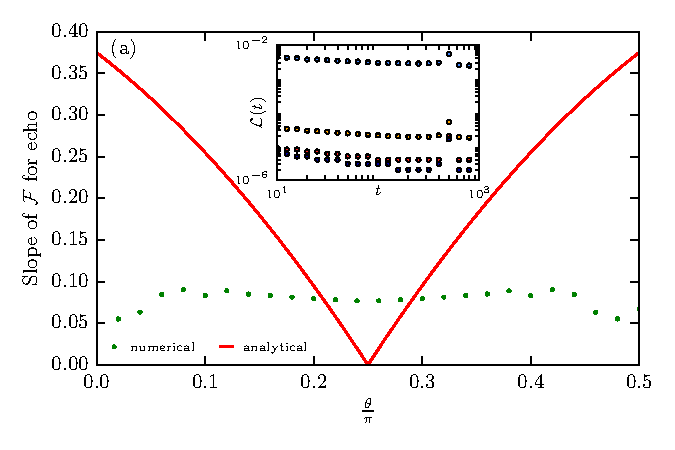
\includegraphics[width=1\columnwidth]{PP_fit.pdf}
    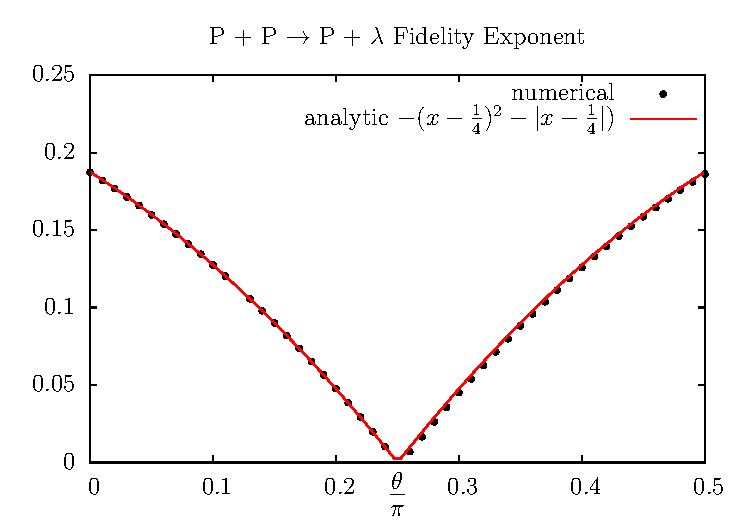
\includegraphics[width=1\columnwidth]{p_p2tan.pdf}
    \caption{The decay exponent of Loschmidt echo (a) and bipartite fidelity (b) in the process $\text{P}+\text{P}\rightarrow\lambda+\text{P}$. The parameters are the same as those in Fig.~\ref{fig:DDNN}. The plot is symmetric with respect to $\theta=0.25\pi$ as predicted. The deviation around $\frac{\pi}{4}$ in (a) is small but visible, see the discussion in the main text. Inset in (a): From the top to bottom, we show the power law decay of Loschmidt echo with $\theta=0.02\pi, 0.12\pi,0.24\pi$ and $0.48\pi$. The finite size effect do not emerge before $t=10^{4}$. We use the same curve fitting method as described for Fig.~\ref{fig:DDDD}.}
    \label{fig:PPPP}
    \todo[inline]{Mao: Put the PPPP for echo; Tianci: make the plots have the same style?}
\end{figure}


%%% Local Variables:
%%% TeX-master: "bCFT_paper"
%%% TeX-PDF-mode: t
%%% End:
